


\documentclass[a4paper]{book}
\usepackage[margin=2cm]{geometry}
\usepackage[T1]{fontenc}
\usepackage[utf8]{inputenc}
%\usepackage{svg}
\usepackage{graphicx}
\usepackage{epstopdf}
\usepackage{amsmath}
\usepackage{listings}

\usepackage{color}
\usepackage{courier}

\definecolor{mygreen}{rgb}{0,0.6,0}
\definecolor{mygray}{rgb}{0.5,0.5,0.5}
\definecolor{mylightgray}{rgb}{0.9,0.9,0.9}
\definecolor{mymauve}{rgb}{0.58,0,0.82}


\usepackage{caption}
\DeclareCaptionFont{white}{\color{white}}
\DeclareCaptionFormat{listing}{\colorbox[cmyk]{0.43, 0.35, 0.35,0.01}{\parbox{\dimexpr\textwidth-2\fboxsep\relax}{#1#2#3}}}
\captionsetup[JAVA]{format=listing,labelfont=white,textfont=white, singlelinecheck=false, margin=0pt, font={bf,footnotesize}}



\lstnewenvironment{JAVA}[1][]
{\lstset{
  language=Java,                   % the language of the code
  backgroundcolor=\color{mylightgray},   % choose the background color; you must add \usepackage{color} or \usepackage{xcolor}
  basicstyle=\footnotesize,        % the size of the fonts that are used for the code
  breakatwhitespace=false,         % sets if automatic breaks should only happen at whitespace
  breaklines=true,                 % sets automatic line breaking
  captionpos=b,                    % sets the caption-position to bottom
  commentstyle=\color{mygreen},    % comment style
  deletekeywords={...},            % if you want to delete keywords from the given language
  escapeinside={\%*}{*)},          % if you want to add LaTeX within your code
  extendedchars=true,              % lets you use non-ASCII characters; for 8-bits encodings only, does not work with UTF-8
  frame=single,                    % adds a frame around the code
  keepspaces=true,                 % keeps spaces in text, useful for keeping indentation of code (possibly needs columns=flexible)
  keywordstyle=\color{blue},       % keyword style
  morekeywords={*,...},            % if you want to add more keywords to the set
  numbers=left,                    % where to put the line-numbers; possible values are (none, left, right)
  numbersep=5pt,                   % how far the line-numbers are from the code
  numberstyle=\tiny\color{mygray}, % the style that is used for the line-numbers
  rulecolor=\color{black},         % if not set, the frame-color may be changed on line-breaks within not-black text (e.g. comments (green here))
  showspaces=false,                % show spaces everywhere adding particular underscores; it overrides 'showstringspaces'
  showstringspaces=false,          % underline spaces within strings only
  showtabs=false,                  % show tabs within strings adding particular underscores
  stepnumber=1,                    % the step between two line-numbers. If it's 1, each line will be numbered
  stringstyle=\color{mymauve},     % string literal style
  tabsize=2,                       % sets default tabsize to 2 spaces
  title=\lstname,                   % show the filename of files included with \lstinputlisting; also try caption instead of title
  #1
}} {}
\author{Stephan Strauss}

\begin{document}

    \title{Spare Time Development - A little guide line for software developing hobbyists}
    \maketitle
    
\part{Introduction}

\chapter{Why this book}

\section{How it started}


The work on this little book in hand started in the summer of 2012 as side product of a little private Java learning and development project. Although absorbed by the daily work in our company, my good friend Claudio Vaccani and my humble self started to work on it in our spare time. 

\section[Requirements]{Requirements to fulfil}

It is a hard job to get a serious development project done as a hobbyist. Especially at least if you plan to read Thomas Mann, Marcel Proust and Adorno at the same time -- just kidding. Therefore we decided not to reach for the stars but to develop a useful little utility, that fulfils several requirements:


\begin{itemize}
\item should be liked on facebook by Richard Wagner and Nietzsche.
\item should be created by god and such heavy he could not pull himself. 
\end{itemize}
Sorry, this was the wrong list, once again, that requirements should be fulfilled:


\begin{itemize}
\item should be based on pure java code (no native JNI code).
\item should have minimal dependencies to other projects. 
\item should be designed first on paper. 
\item should have a foreseeable finalization.
\item time constraints should be kept minimal - the learning effect maximal. 
\end{itemize}

To be honest, we never believed that we could achieve a final product but we wanted to learn and as much as possible and therefore defined the requirements as such. 

\section{Learning by doing}

I learned already some years before with another friend and former colleague Ralf Gautschi the basics of the java language using several books that I will list at the end of this chapter. Therefore this project as described in this book was more concerned about good design and patterns, about unit testing and re-factoring, about agile programming and other streams and temporary fashions - not so much about the java language itself. 

With not much knowledge but with a unbreakable will we started and ended successfully the project: 
The resulting little story is worth telling and therefore written down in this little cheap Amazon book for Amazons.

Because the corresponding source code is probably not the best seen in software 
industry,  the self-critical aspect is the center of this book. I think we learned a lot
, especially by criticizing our own result.

Ralf Gautschi is now principle engineer at Microsoft, Zuerich. Claudio and me are still working for Synopsys AG. We are both located in Zurich and work in R\&D. 
   
   
The tool developed (it's working name was TEME) is used to measure precisely distances and aeras   
   
\chapter{Drawables}

\section{The \texttt{Drawable} Interface}

The basic property of all objects that should be drawn in the \texttt{TEMView} 


%\begin{JAVA}[float=htbp, label=Drawable,caption=The Drawable Interface all \texttt{Drawables} are implemented against]
\begin{JAVA} [label=Drawable,caption=The Drawable Interface all \texttt{Drawables} are implemented against]
public interface Drawable  {	
	public void paint(Graphics2D graphicsContext, AffineTransform transformation); 		
	public boolean contains(int x, int y);	
}
\end{JAVA}


\section{The Reference Scale Drawable}

    

	\begin{figure}[htbp]
  		\centering
  		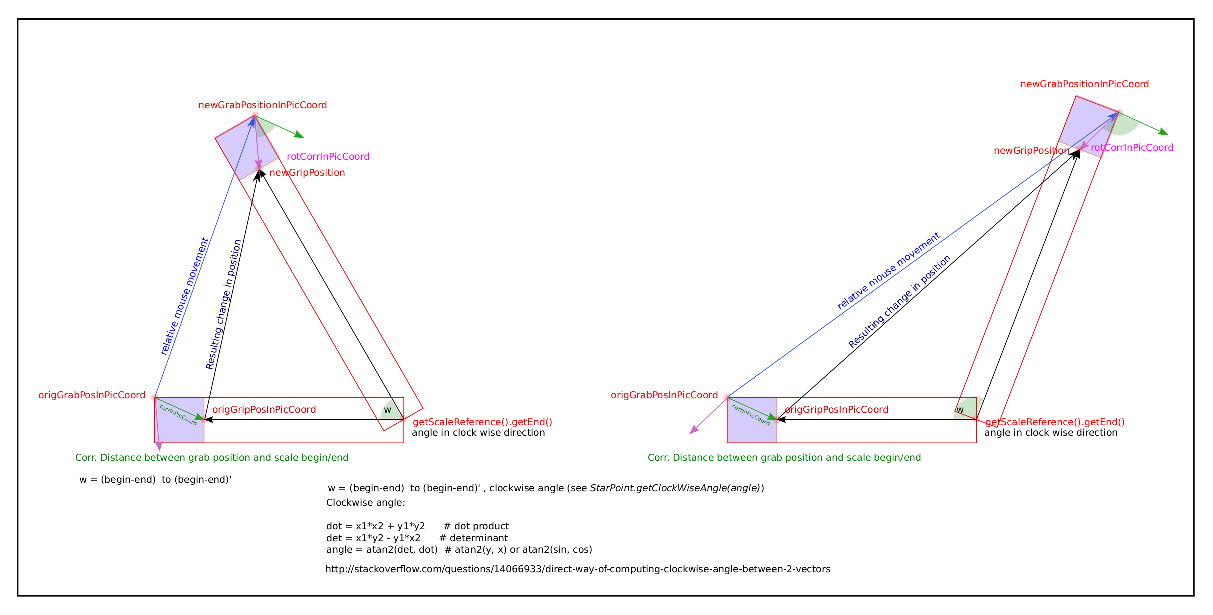
\includegraphics[width=\textwidth]{scaleDescription.eps}
  		\caption{Calculation of a new grip position as function of a relative repositioning of the mouse 	pointer}
	\end{figure}


\end{document}
